\documentclass{scrartcl} 
% Include all project wide packages here.
\usepackage{fullpage}
\usepackage{polyglossia}
\setmainlanguage{dutch}
\usepackage{csquotes}
\usepackage{graphicx}
\usepackage{epstopdf}
\usepackage{pdfpages}
\usepackage{caption}
\usepackage[list=true]{subcaption}
\usepackage{float}
%\usepackage{mathtools}
\usepackage{standalone}
\usepackage{import}
\usepackage{tocloft}
\usepackage{wrapfig}
\usepackage{authblk}
\usepackage{array}
\usepackage{booktabs}
\usepackage[toc,page,title,titletoc]{appendix}
\usepackage{xunicode}
\usepackage{amsmath}
\usepackage{fontspec}
\usepackage{unicode-math}
\usepackage[
    backend=bibtexu,
	texencoding=utf8,
bibencoding=utf8,
    style=ieee,
    sortlocale=nl_NL,
    language=auto
]{biblatex}
\usepackage{listings}
\newcommand{\includecode}[3][c]{\lstinputlisting[caption=#2, escapechar=, style=#1]{#3}}
\newcommand{\superscript}[1]{\ensuremath{^{\textrm{#1}}}}
\newcommand{\subscript}[1]{\ensuremath{_{\textrm{#1}}}}


\newcommand{\chapternumber}{\thechapter}
\renewcommand{\appendixname}{Bijlage}
\renewcommand{\appendixtocname}{Bijlagen}
\renewcommand{\appendixpagename}{Bijlagen}

\usepackage[hidelinks]{hyperref} %<--------ALTIJD ALS LAATSTE

\renewcommand{\familydefault}{\sfdefault}

\setmainfont[Ligatures=TeX]{Myriad Pro}
\setmathfont{Asana Math}
\setmonofont{Lucida Console}

\usepackage{titlesec, blindtext, color}
\definecolor{gray75}{gray}{0.75}
\newcommand{\hsp}{\hspace{20pt}}
\titleformat{\chapter}[hang]{\Huge\bfseries}{\chapternumber\hsp\textcolor{gray75}{|}\hsp}{0pt}{\Huge\bfseries}
\renewcommand{\familydefault}{\sfdefault}
\renewcommand{\arraystretch}{1.2}
\setlength\parindent{0pt}

%For code listings
\definecolor{black}{rgb}{0,0,0}
\definecolor{browntags}{rgb}{0.65,0.1,0.1}
\definecolor{bluestrings}{rgb}{0,0,1}
\definecolor{graycomments}{rgb}{0.4,0.4,0.4}
\definecolor{redkeywords}{rgb}{1,0,0}
\definecolor{bluekeywords}{rgb}{0.13,0.13,0.8}
\definecolor{greencomments}{rgb}{0,0.5,0}
\definecolor{redstrings}{rgb}{0.9,0,0}
\definecolor{purpleidentifiers}{rgb}{0.01,0,0.01}


\lstdefinestyle{csharp}{
language=[Sharp]C,
showspaces=false,
showtabs=false,
breaklines=true,
showstringspaces=false,
breakatwhitespace=true,
escapeinside={(*@}{@*)},
columns=fullflexible,
commentstyle=\color{greencomments},
keywordstyle=\color{bluekeywords}\bfseries,
stringstyle=\color{redstrings},
identifierstyle=\color{purpleidentifiers},
basicstyle=\ttfamily\small}

\lstdefinestyle{c}{
language=C,
showspaces=false,
showtabs=false,
breaklines=true,
showstringspaces=false,
breakatwhitespace=true,
escapeinside={(*@}{@*)},
columns=fullflexible,
commentstyle=\color{greencomments},
keywordstyle=\color{bluekeywords}\bfseries,
stringstyle=\color{bluestrings},
identifierstyle=\color{purpleidentifiers}
}

\lstdefinestyle{vhdl}{
language=VHDL,
showspaces=false,
showtabs=false,
breaklines=true,
showstringspaces=false,
breakatwhitespace=true,
escapeinside={(*@}{@*)},
columns=fullflexible,
commentstyle=\color{greencomments},
keywordstyle=\color{bluekeywords}\bfseries,
stringstyle=\color{redstrings},
identifierstyle=\color{purpleidentifiers}
}

\lstdefinestyle{xaml}{
language=XML,
showspaces=false,
showtabs=false,
breaklines=true,
showstringspaces=false,
breakatwhitespace=true,
escapeinside={(*@}{@*)},
columns=fullflexible,
commentstyle=\color{greencomments},
keywordstyle=\color{redkeywords},
stringstyle=\color{bluestrings},
tagstyle=\color{browntags},
morestring=[b]",
  morecomment=[s]{<?}{?>},
  morekeywords={xmlns,version,typex:AsyncRecords,x:Arguments,x:Boolean,x:Byte,x:Char,x:Class,x:ClassAttributes,x:ClassModifier,x:Code,x:ConnectionId,x:Decimal,x:Double,x:FactoryMethod,x:FieldModifier,x:Int16,x:Int32,x:Int64,x:Key,x:Members,x:Name,x:Object,x:Property,x:Shared,x:Single,x:String,x:Subclass,x:SynchronousMode,x:TimeSpan,x:TypeArguments,x:Uid,x:Uri,x:XData,Grid.Column,Grid.ColumnSpan,Click,ClipToBounds,Content,DropDownOpened,FontSize,Foreground,Header,Height,HorizontalAlignment,HorizontalContentAlignment,IsCancel,IsDefault,IsEnabled,IsSelected,Margin,MinHeight,MinWidth,Padding,SnapsToDevicePixels,Target,TextWrapping,Title,VerticalAlignment,VerticalContentAlignment,Width,WindowStartupLocation,Binding,Mode,OneWay,xmlns:x}
}

%defaults
\lstset{
basicstyle=\ttfamily\small,
extendedchars=false,
numbers=left,
numberstyle=\ttfamily\tiny,
stepnumber=1,
tabsize=4,
numbersep=5pt
}
\addbibresource{../library/bibliography.bib}

\author{Groep 1 (DaC)}
\title{EPO-3 "Maak een Chip" Project Plan}

\date{14-10-2013}

\begin{document}
\pagenumbering{roman}
\maketitle
\vspace{80 mm}
\section*{Samenvatting}
In dit verslag zal de opzet van het project uitgelegd worden. Het uiteindelijke resultaat van dit project is het maken van een functionele chip, waarbij de chip volledig zal worden gespecificeerd, ontworpen en gesimuleerd door en groep studenten. De chip zal gefabriceerd worden door DIMES. 
\newpage
\setlength{\cftbeforetoctitleskip}{-3em}

\tableofcontents
\newpage
\pagenumbering{arabic}
\section{Achtergrond}
Het project "Maak een Chip"\ is een vervolg op de projecten uit het eerste jaar van de bachelor Electrical Engineering, waarbij de nadruk is gelegd op het gestructureerd hierarchisch ontwerpen van een chip en zoals bij elk project het samenwerken in een groep. Dit wordt gedaan met een groep van 9 bsc electrical engineering studenten. Wanneer het ontwerp af is, wordt deze in het 2e semester tot werkelijkheid gebracht in de chipfabriek DIMES en in het 4de kwartaal zal de chip af zijn en getest kunnen worden. Bij dit project zal de kennis van bepaalde vakken zoals lineaire schakelingen, halfgeleiders en versterkerschakelingen uit het eerste jaar electrical engineering toegepast worden om zo een goed en werkend product te krijgen.

\section{Projectopdracht}
Het uiteindelijke resultaat dat moet worden bereikt met dit project is het maken van een correct ontwerp van een chip met alle bijbehorende stappen. Om dit te kunnen bereiken dienen een aantal doelen bereikt te worden;
\begin {itemize}
\item Het ontwerpen aan de hand van algemene productspecificaties met randvoorwaarden.
\end {itemize}
\quad Het is belangrijk voor het ontwerpen van de chip, dat de productspecificaties met randvoorwaarden zo goed en duidelijk mogelijk worden gespecificeerd. 
Zo zal het ontwerpen van de chip makkelijker verlopen en bepaalde problemen en limitaties zullen voor de deadline verholpen kunnen worden.
\begin {itemize}
\item Het ontwerp systematisch en hierarchisch opstellen.
\end {itemize}
\quad Door het ontwerp systematisch en hierarchisch te maken hou je een duidelijke structuur in het geheel. Aanpassingen zoals het opzoeken en repareren van fouten, het toevoegen van modules en het aanpassen van modules zullen door deze werkwijze veel gemakkelijker zijn.
\begin {itemize}
\item Het ontwerp analyseren 
\end {itemize}
\quad Het is belangrijk om het ontwerp op verschillende niveau's te analyseren met behulp van simulaties, prototyping en metingen. Op deze manier kan worden getest of het ontwerp ook op switch-level en transistor niveau mogelijk is. Wanneer dit niet zo is kan het ontwerp worden aangepast zodoende dat dit wel mogelijk is.
\begin {itemize}
\item Het ontwerp opstellen aan de hand van verscheidene modellen
\end {itemize}
\quad Bij het modelleren van het ontwerp is het belangrijk om de beperkingen van het gebruikte model in de gaten te houden, zodat er rekening kan worden gehouden met uitkomsten die het model niet kan verklaren. Om deze reden is het handig met behulp van verschillende modellen te modeleren zodat hierover een duidelijk beeld onstaat.
\begin {itemize}
\item Het ontwerp testbaar maken
\end {itemize}
\quad Bij het ontwerpen van de chip moet ook op de testbaarheid van het ontwerp gelet worden. Wanneer dit niet gebeurd zal het ontwerp niet goed te simuleren zijn en zal het moeilijk zijn om fouten en beperkingen te vinden in het ontwerp.

\section{Projectactiviteiten}
\begin{itemize}
\item Maken van het Project Plan
\item Specificaties \&  Randvoorwaarden bepalen voor een chip.
\item Haalbaarheid van de te ontwerpen chip bepalen.
\item Het gekozen ontwerp opdelen in functieblokken.
\item IC ontwerpen \& simuleren.
\item De IC prototypen op FPGA.
\item Tussenrapport schrijven.
\item Het eindverslag schrijven.
\end{itemize}

\section{Randvoorwaarden}
\begin{itemize}
\item Het project loopt van 9 Sept. 2013 tot 15 Januari 2014. 
\item Het project dient gedaan worden in groepen van 7-10 personen.
\item De chip wordt geleverd door de TU Delft en gefabriceerd door DIMES.
\item Het Altera DE1/DE2 FPGA-bordje voor prototyping wordt geleverd door de TU Delft.
\item Alle software ontwerptools worden geleverd door de TU Delft.
\end{itemize}

%\section{Specificaties}
%\subsection {Functionele Eisen}
%
%\subsection {Randvoorwaarden}
%\begin {itemize}
%\item De algemene technische randvoorwaarden zijn bepaald in hoofdstuk 11.8 "\Algemene Technologische Randvoorwaarden"  van het EPO-3 Handleiding/cite{epo3-manual}
%\item Beeldresolutie van 640x480 in 16 kleuren.
%\end{itemize}

\section{Producten}
\begin{itemize}
\item Het Projectplan
\item Specificaties \& Randvoorwaarden van GPU
\item Functieblokschema Ontwerp GPU
\item Ontwerp IC
\item Het Tussenrapport
\item Het Chip Ontwerp
\item Bestanden van de volledige Chip
\item Het Eindverslag
\end {itemize}

\section{Kwaliteit}
Alle ontwerpbeslissingen worden met minimaal 50\% van de groep besproken.
\\Het resultaat van een bepaalde module wordt na uitwerking besproken met de groep om zekerheid te verkrijgen van zijn functionaliteit.
\\Alle modules moeten in VHDL geschreven worden en er moet rekening gehouden worden met de VHDL restricties. Alle modules worden gesimuleerd vervolgens gesynthetiseerd en tot slot \\wordt er place en route gebruikt om zekerheid te verkrijgen dat de chip op alle niveau's, namelijk VHDL, switch level en transistor, volledig functioneel is.
\\De chip moet geprototyped worden op de FPGA chip om zo er zeker van te zijn dat de chip in theorie werkt.

\section{Projectorganisatie}
\begin {tabular}{|c|c|}
\hline
Marian Bartek & Tutor\\
\hline
Joris Coenen & Studentmentor\\
\hline
Efraïm Eland & Projectlid\\
\hline
Robin Hes & Voorzitter\\
\hline
Tu Hoang & Projectlid\\
\hline
Kees Hogenhout & Projectlid\\
\hline
Alex Janssen & Projectlid\\
\hline
Jorden Kerkhof & Projectlid\\
\hline
Peter Stijnman & Projectlid\\
\hline
Xenia Wesdijk & Projectlid\\
\hline
Erwin de Haan & Projectlid\\
\hline
\end {tabular}
\\
\\Er zullen elke middag twee vergaderingen plaatsvinden. Een openingsvergadering om 8:50 en een afsluitende vergadering om 12:30.
Alle documentatie zal geplaatst worden op github met dropbox als backup.
Alle officiële documentatie zullen gemaakt worden in Latex en gepubliceerd worden in pdf formaat.
\newpage
\section{Planning}
Zie Figuur 1.
 \begin{figure}[H]
\centering
	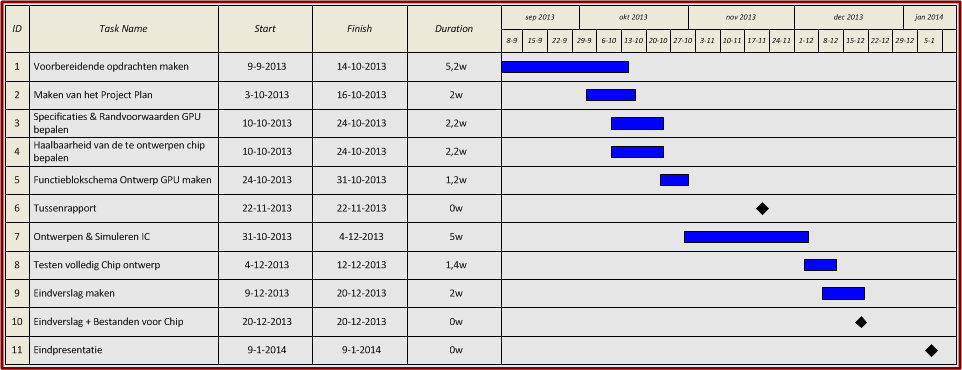
\includegraphics[width=18cm]{Planner}
	\caption{De voorlopige planning}
	\label{fig:planning}
\end{figure}

\section{Risico's}
Het grootste risico bij dit project is dat de gekozen specificaties en randvoorwaarden niet gehaald kunnen worden, omdat het met het aantal transistoren op de chip niet mogelijk is om al de functies te maken. Om dit te voorkomen zal er tijdens het bepalen van de specificaties en randvoorwaarden kleinschalige simulaties worden gedaan met het test FPGA-bordje om echte haalbaarheid te testen. Zo zal er voor de implementatie fase al zeker zijn van wat er tenminste haalbaar is.
\\Daarnaast zal de planning ook een rol spelen in de haalbaarheid van het project, omdat zonder een duidelijke planning bepaalde aspecten van het gekozen ontwerp niet goed uitgevoerd kunnen worden en dan zal het eindproduct niet werken.
\\Nog een risico is dat de vertaling van code naar hardware niet klakkeloos zal verlopen. Er kunnen problemen onstaan, omdat bepaalde gedeeltes van de code niet goed overgezetzijn en dan zal het eindproduct ook niet werken.
\\Een ander risico is dat bij het uiteindelijke product sommige verbindingen tussen transistoren niet goed zijn aangelegd, maar de chip wordt drie maal gefabriceerd, dus die kans zal erg klein zijn.

\newpage
\section{Bibliografie}
\printbibliography

\end{document}
